\section{Mixed sediments}%\footnote{This chapter has been written by D. Phan van Bang, Lan and Villaret}

\label{ch:mixed}

\subsection{Sediment bed composition}

\subsubsection{Characteristics of each class}
Sand-mud mixture can be represented in \sisyphe by using two classes of bed
sediments (\texttt{NSICLA= 2}). This recent developments available in release 6.3
require further testing and improvement. 
The \textbf{first class (noted 1) is non-cohesive} and represented by its grain
diameter $D_1$ and can be transported as bed-load or suspended load. The
settling velocity $w_{s1}$ is a function of the relative sediment density
($s=1.65$) and grain diameter $D_1$. So far we assume only suspended load,
which implies that the model is devoted to mixtures of fine sand grains and
mud.

The \textbf{second class (noted 2) is cohesive}, grain diameter $D_2$ less than $60$
mm. The settling velocity $w_{s2}$ is a function of flocs properties which
differs from the individual cohesive particles, and needs to be specified. 

\subsubsection{Vertical structure of the sediment bed}
The vertical structure can be stratified as for pure mud. The bed is
discretized into vertical layers up to a maximum number of layers (\texttt{NOMBLAY <20}). 
Each layer is characterized by a constant value of the mass
concentration for the mud, which can be specified in the steering file ($C_{si}$ for \texttt{i=1, NOMBLAY}). 

\begin{bclogo}[couleur = blue!10, arrondi = 0.10, logo = \bcattention]{\textsf{Attention}}
The mass concentration of the mud component is defined for the mud
only (i.e. mass of sediments per volume of mud). The initial bed layer
thicknesses can be specified in subroutine \texttt{init\_mixte.f}, and varies as the
bed undergoes erosion/deposition. The consolidation of sand/mud mixture is
not yet developed.
\end{bclogo}

The time and spatial variation in the sediment composition is obtained by
variation in the composition of each layers (Percent of the mud and mass of
sand per layers). 

\begin{figure}[H]
\begin{center}
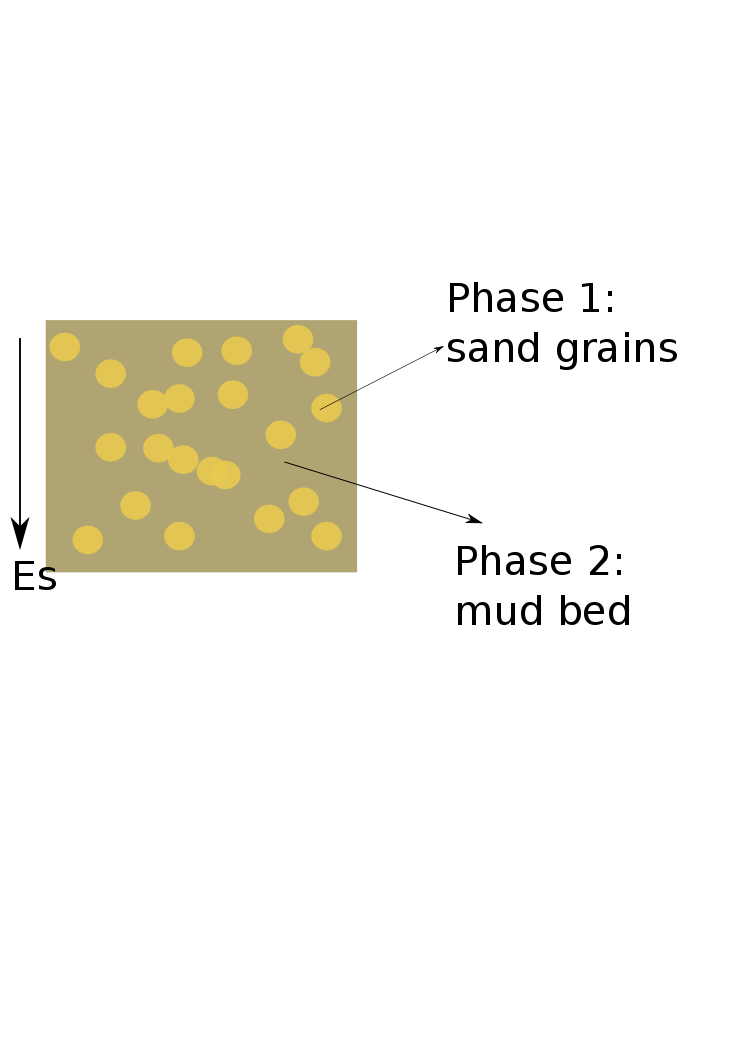
\includegraphics[scale=0.3,angle=0]{graphics/mudsand_1.png}
\caption{Percent of mud/sand mixture for layer $j$.}\label{fig:mudsand1}
\end{center}
\end{figure}

The composition of the sediment bed depends on the percent of each class ($P_1, P_2$) needs to be specified. In consistency with the algorithm for sand grading effects, $P_i$ represents the volume of class $i$ divided by
the total volume, such that $P_1+P_2 =1$:
\begin{equation*}
P_i = \frac{V_i}{V_t}, 
\end{equation*}
where $V_i$ is the volume occupied by component $i$, and $V_t=V_1+V_2$, the total volume. The total thickness of the layer $j$ is decomposed into $Es= Es_1 + Es_2$, with $Es_i = p_i Es$. The total mass of the sand-mud mixture ($M_t$) is:
\begin{equation*}
M_{t} =C_{s} V_{2} +\rho _{s} V_{1} =\left( C_{s} P_{2} +\rho _{s} P_{1}
\right) V_{t} 
\end{equation*}
with $\rho_s = 2650$ kg/m$^{3}$ (constant sand density), while
for the mud, $C_s$ depends on the consolidation state and is constant per
sediment bed layer. It is specified by using keyword \texttt{MUD CONCENTRATION PER
LAYER}.

\subsubsection{Mass balance}
The total mass of the sand-mud mixture ($M_t$) is:
\begin{equation*}
M_t =C_s V_2 + \rho_s V_1 = \left(C_sP_2+\rho_sP_1\right)V_t. 
\end{equation*}
We define for each class the mass per surface area and per layer:
\begin{equation*}
MS\_VASE=\left\{\begin{array}{l}
Cs\,P_2\,Es \\
\rho_s\,P_1\, Es
\end{array}
\right. 
\end{equation*}

For the mass balance of the mud phase (phase 2):
\begin{equation*}
M_2 =\sum\limits_{i=1,Npoin}
\left[\underbrace{\sum\limits_{j=1,Nomblay}P_2\,Cs\,Es}_{MS\_VASE}\right]_j S_i 
\end{equation*}%

\subsubsection{Initialization}
The initial percent of each class ($p_1, p_2$) needs to be specified.
The keyword \texttt{INITIAL FRACTION FOR PARTICULAR SIZE CLASS} can be applied, if
the initial distribution is constant (per layer and per node). In the mass balance for each class, the total mass per unit surface area must account for the fraction of each class:

For the type of sediments:
\medskip
\begin{bclogo}[couleur=blue!10,arrondi=0.1, logo=\bcinfo]{Keywords}
\begin{itemize}
\item {\ttfamily MIXED SEDIMENT = YES} ({\ttfamily = NO}, default option)
\item {\ttfamily COHESIVE SEDIMENTS = YES} ({\ttfamily = NO}, default option)
\item {\ttfamily NUMBER OF SIZE-CLASSES OF BED MATERIAL = 2} ({\ttfamily NSICLA}) 
\item {\ttfamily SEDIMENT DIAMETERS = D1, D2} (for non-cohesive sediments {\ttfamily D1>6.0E-5}, for cohesive sediments {\ttfamily D1<6.0E-5}.)
\item {\ttfamily SETTLING VELOCITIES = $ws_1$, $ws_2$} 
\end{itemize}
\end{bclogo}

For the bed composition:
\medskip
\begin{bclogo}[couleur=blue!10,arrondi=0.1, logo=\bcinfo]{Keywords}
\begin{itemize}
\item {\ttfamily NUMBER OF LAYERS OF THE CONSOLIDATION MODEL} ({\ttfamily NOMBLAY = 10}, default option)
\item {\ttfamily MUD CONCENTRATION PER LAYER} (in kg/m$^3$, {\ttfamily CONC\_VASE=
50.; 100.;...}, default option)
\item {\ttfamily INITIAL FRACTION FOR PARTICULAR SIZE CLASS = $p_1$; $p_2$} 
\end{itemize}
\end{bclogo}

\subsection{Erosion/deposition fluxes}
The erosion/deposition fluxes now depends on the mass pourcentage $\%$ of each class in
the surface layer (Panagiotopoulos et al., 1997). If the mass percent of the
mud class is greater than $50\%$, the bed is considered as pure cohesive and
the erosion/deposition laws follow the Partheniades classical law. (see
below for the calculation of the bed shear strength in a sand/mud mixture).

If the mud percentage is less than $30\%$, the bed is considered as non
cohesive, and has little effect on the bed shear strength. Once sediment particles have been put in suspension, they are transported independently, by solving for each class, a transport equation for the
volume concentration of the individual sediment particles (deflocculated)
defined as:

\begin{equation*}
C_i =\frac{C_i}{\rho_s} 
\end{equation*}

Mud flocs in suspension

Sand grains in suspension

\begin{equation*}
\frac{\partial C_i}{\partial t} + U_{conv}\frac{\partial C_i}{\partial
x} +V_{conv} \frac{\partial C_i}{\partial y} =\left[\frac{\partial }{%
\partial x} \left(\epsilon_s\frac{\partial C_i}{\partial x} \right) +%
\frac{\partial }{\partial y} \left( \epsilon_s\frac{\partial C_i}{%
\partial y} \right) \right] +\frac{(E_i - D_i)}{h} 
\end{equation*}%
The erosion flux is determined for each class of sediments as a function of
the bed composition. The deposition flux $D= w_{si} C_i$ is treated implicitly.

\begin{figure}[H]
\begin{center}
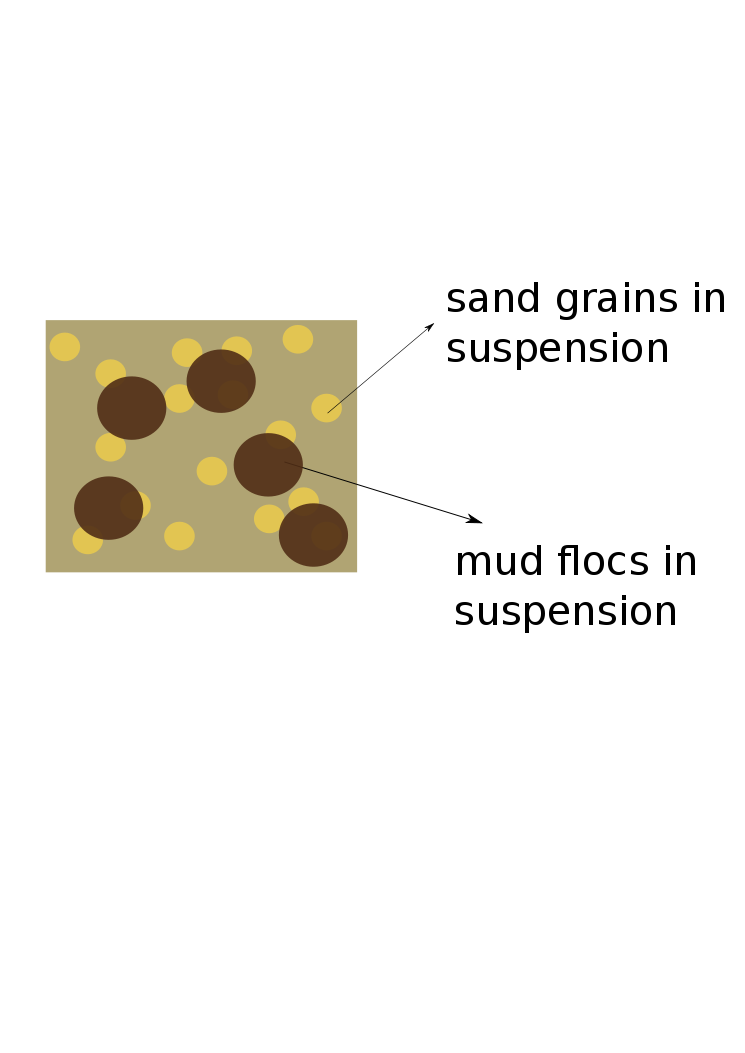
\includegraphics[scale=0.3,angle=0]{graphics/mudsand_2.png}
\caption{Concentration of the individual sediment particles.}\label{fig:mudsand2}
\end{center}
\end{figure}

\subsection{Erosion law for sand mud mixture}
The rate of erosion is based on the Partheniades erosion law, where the
critical bed shear strength of the mud class depends on the consolidation
state.

The bed shear strength of the sand mud mixtures depends on the \% of mud ($P_2$ at the surface top layer). We follow here the method of Waeles (2005, [36]). The erosion rate $E_{(1+2)}$ is calculated for the mixture and then for each class $E_i$:
\begin{equation*}
E_i = P_i E_{(1+2)}.
\end{equation*}%
\begin{itemize}
\item If $C>50\%$ then mud dominant. We apply the Krone erosion law:

\begin{equation*}
E_{(1+2)} = \left\{\begin{array}{ll}
M\left[\left(\frac{u_*}{u_{*e}} \right)^2-1\right]\quad & \text{if}\,\,\tau_b=\rho u_*^2>\tau_{ce}=\rho u_{*e}^2\\  
0\quad & \text{if}\,\,\tau_b<\tau_{ce}
\end{array}
\right. 
\end{equation*}

\item If C\texttt{<}30\%: sand dominant. We apply the Zyserman and Fredsoe equilibrium concentration:
\begin{equation*}
E_{(1+2)} = w_{s1} C_{eq}\quad\text{for}\quad tau_b=\rho u_*^2>\tau_{ce}=\rho u_{*e}^2 
\end{equation*}

\item If $30\%<C<50\%$: intermediate range. We assume a linear interpolation of erosion rates for each class.
\end{itemize}

\subsection{Bed evolution}
The bed evolution for both phases is calculated differently following the
method for pure mud or pure sand; This is not entierely correct and should
be modified in the near future.

\subsubsection{For sand (phase 1)}
We assume the first layer to be greater than the active layer thickness,
such that the sand percent can be considered to be constant and equal to the
percent of the top layer.

\begin{equation*}
P_1 dZ_{f1} =(D_1 - E_1)\,Dt 
\end{equation*}

In this mass balance for sand, we do not consider the void ratio, since it
is entirely filled by the fine sediments (the volume concentration of the
sand phase is $1$, instead of $(n-1)$, where $n$ is the bed porosity in case of
either pure sand or sand mixtures).

If there is net erosion $(E_1-D_1) > 0$, the first layer $Es_1$ is
decreased $Es_1=Es_1-P_1dZf_1$ which is only correct if $Es_1-P_1dZf_1>0$.

If there is net deposition $(D_1-E_1)>0$, the sediment is deposited in
the first top layer $Es_1$ is increased $Es_1=Es_1-P_1dZf_{1}$.

\subsubsection{For mud (phase 2)}
We follow the method described in part. The top layers are successively
eroded until we match the erosion flux. In case of deposition $(D_2-E_2)>0$, the sediment is deposited in the
top layer:
\begin{equation*}
P_2 C s_2 \,DZf_{f_2} =\rho_s (D_2 - E_2) Dt 
\end{equation*}

The top layer thickness is increased in order to match $Es_2= Es_2+dZf_2$.
In case of erosion the procedure consist in determining the maximum layer to
be eroded:

\begin{equation*}
\sum\limits_{j=1}^{j\max -1} Ms_{2}(j) < \rho_s(E_2-D_2)Dt< \sum\limits_{j=1}^{j\max } Ms_2(j) 
\end{equation*}

All top layers (up to $jmax-1$) are emptied: for the last one, the mass balance is now computed as:
\begin{equation*}
\sum\limits_{j=1}^{j\max -1} Ms_2(j) + dEs_2(j\max)Cs(j\max)=\rho_s(E_2-D_2)Dt 
\end{equation*}

\subsubsection{Reactualisation of the bed composition}
The percent of each class of sediment needs to be recalculated (end of
suspension main):
\begin{equation*}
P_i =\frac{Es_i}{Es}, 
\end{equation*}
with $Es= Es_1+Es_2$.

%\section*{ Conclusions}

%This report presents recent developments in SISYPHE 6.2 for the treatment of
%cohesive sediment transport (for erosion, deposition, bed evolution and
%consolidation algorithm). Preliminary features for mixed sediments are also
%described, although this part is still under development and definitely
%needs further validation based on well documented data sets. The test cases
%for cohesive sediments are based on experiments on the Gironde mud and
%further applications under in-situ conditions can be found in Van's PhD
%thesis (2012).\newline

%\subsection*{References}



